\section{Documentação Doxygen e o Doxywizard}

O Doxygen é um gerador de documentação, ou seja, uma ferramenta utilizada para a redação de documentos acerca de um software. O conteúdo da documentação é escrito no corpo do código, o que facilita o referenciamento de partes do código no documento.

\subsection{Uso}

Além de aceitar a sintaxe do Javadoc, o Doxygen suporta marcações de documentação usadas no Qt toolkit e a sua saída pode ser em HTML, CHM, RTF, PDF, LaTeX, PostScript ou man pages (páginas de manual).

\subsection{Doxywizard}

Doxywizard é uma interface para a configuração e o uso do Doxygen.
Ao ser inicializado, o Doxywizard mostrará sua janela principal. Algumas diferenças visuais poderão ser notadas nos diferentes Sistemas Operacionais utilizados (caso suportados). 
\begin{figure}[!htb]
\centering
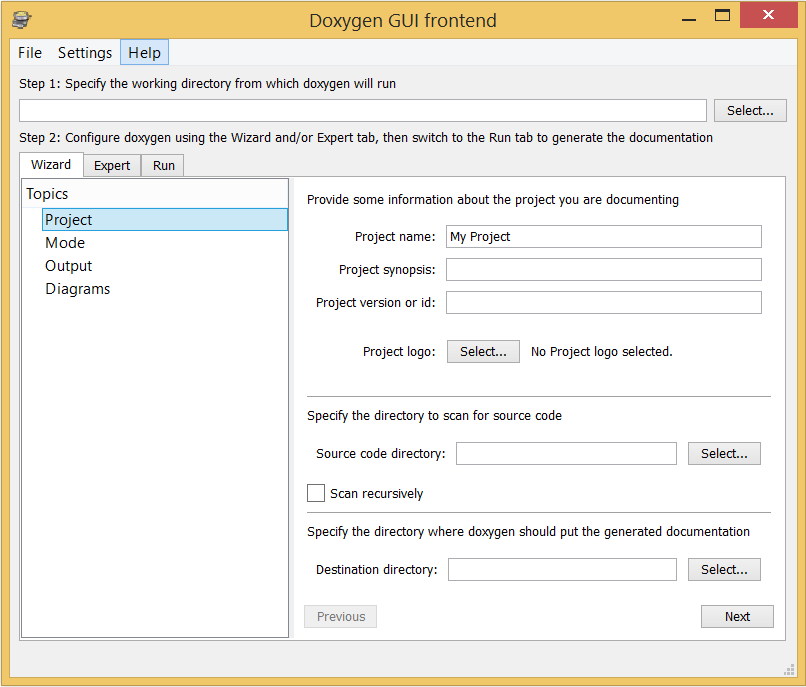
\includegraphics[width=7cm]{./include/chapters/sections/soft/section4/img/janela.png}
\caption{Janela Principal}
\end{figure}\\
Esta janela mostra os passos para realizar a configuração e a utilização do Doxygen. O primeiro passo é escolher uma das opções de configuração:
\begin{itemize}
\item  Wizard: Utilizado para configurar rapidamente as opções mais importantes e manter o restante das opções em seus padrões;
\item  Expert: Utilizado para ter acesso a todas as opções configurações;
\item  Run: Utilizado para gerar a documentação após realizadas as configurações.
\end{itemize}
É possível (e comum) realizar uma configuração básica utilizando o Wizard e realizar ajustes específicos no modo Expert.
\subsubsection{Wizard}
A aba Wizard comummente está selecionada ao iniciar-se o Doxygen, podendo ser vista na Figura 2.9. 
\subsubsection{Project}
Quando selecionada, a aba Wizard permite acesso às seguintes opções:
\begin{itemize}
\item  Determinar informações como nome, uma pequena sinopse, versão do código e logotipo do projeto;
\item  Especificar o diretório do código;
\item  Especificar o diretório alvo do documento gerado.
\end{itemize}
\subsubsection{Modes}
\begin{figure}[!htb]
\centering
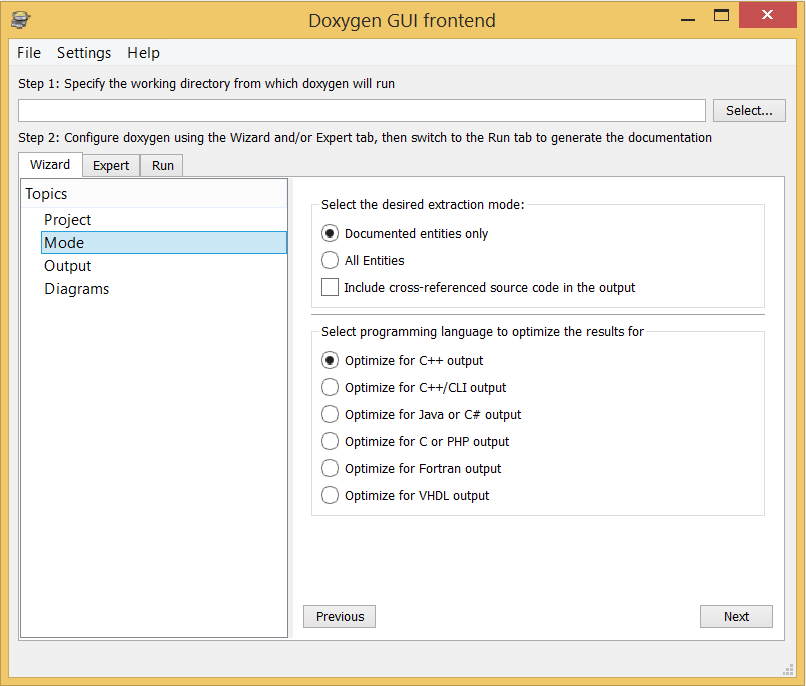
\includegraphics[width=6.5cm]{./include/chapters/sections/soft/section4/img/mode.png}
\caption{Modes}
\end{figure}
No tópico Modes é possível configurar algumas opções referentes à linguagem de programação utilizada.
\subsubsection{Output}
Tópico onde são realizadas configurações (como formato, cores e tipos) do documento gerado.
\begin{figure}[!htb]
\centering
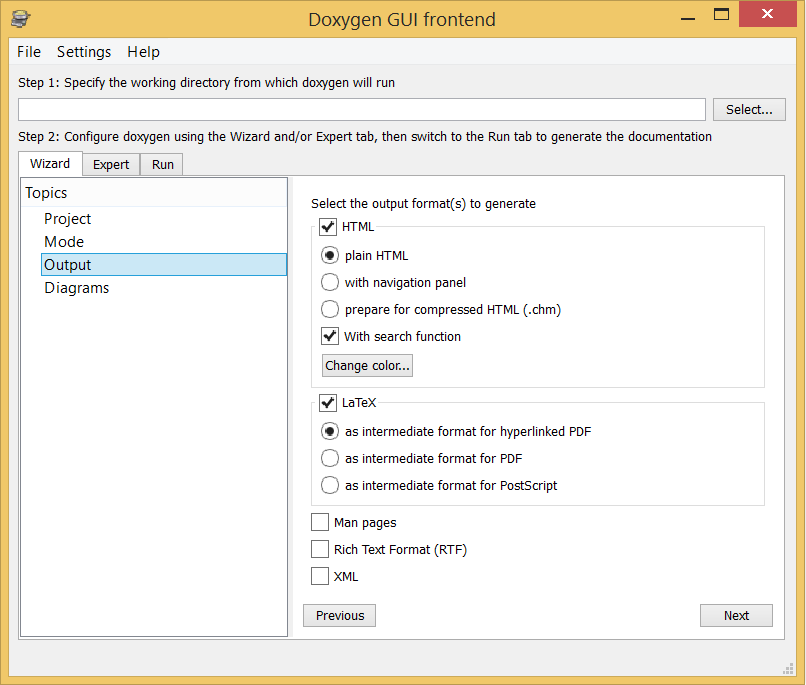
\includegraphics[width=6.5cm]{./include/chapters/sections/soft/section4/img/output.png}
\caption{Outputs}
\end{figure}
\subsubsection{Diagrams}
Tópico relacionado à diagramas.
\begin{figure}[!htb]
\centering
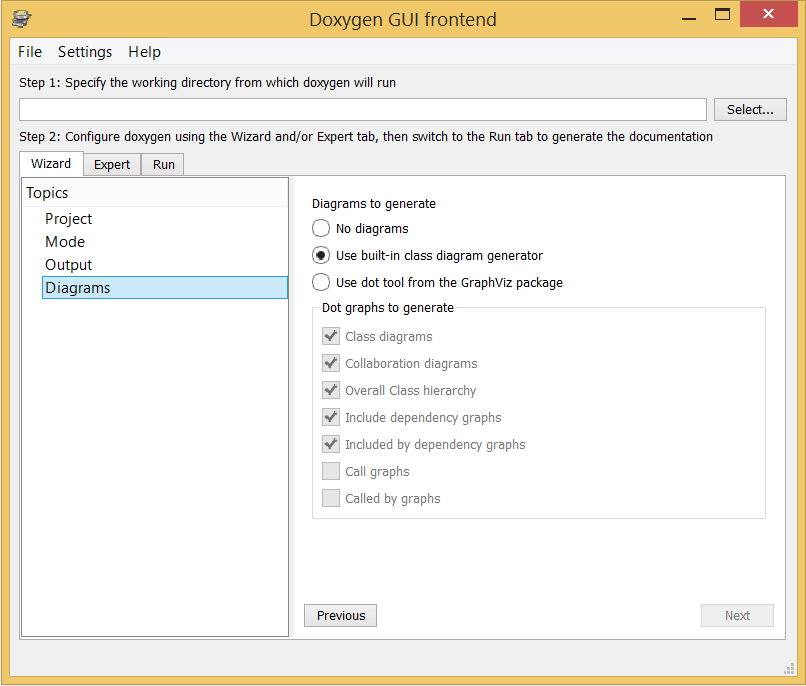
\includegraphics[width=7.2cm]{./include/chapters/sections/soft/section4/img/diagrams.png}
\caption{Diagramas}
\end{figure}

\subsubsection{Expert}

A aba Expert oferece opções de configuração mais detalhadas e avançadas.
\begin{figure}[!htb]
\centering
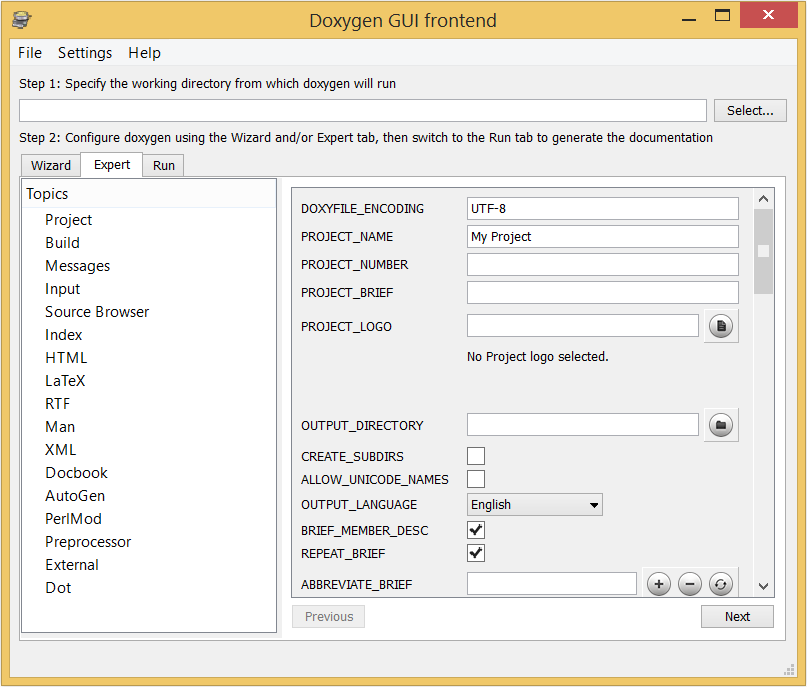
\includegraphics[width=7.2cm]{./include/chapters/sections/soft/section4/img/expert.png}
\caption{Expert}
\end{figure}

\subsubsection{Run}

A aba Run permite a geração da documentação.
\begin{figure}[!htb]
\centering
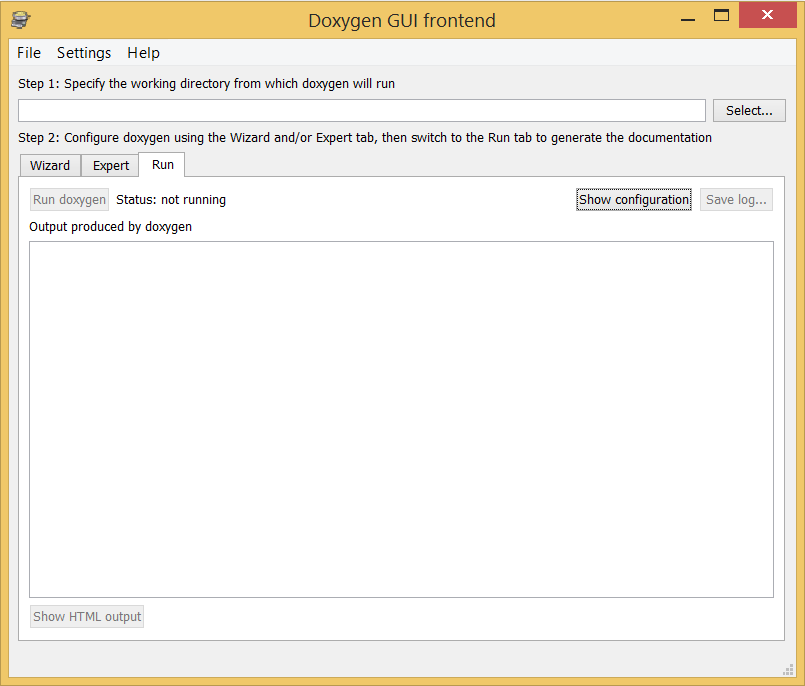
\includegraphics[width=7.2cm]{./include/chapters/sections/soft/section4/img/run.png}
\caption{Run}
\end{figure}